\chapter{TLS echoservice}

TLS provides security and data integrity


Diffrent kind of security is intended;
\begin{enumerate}
 \item Integrity (data is not manipulated along the transmission)
 \item Confidentiality 
 \item Authenticity (Server and client sided)
 \item Authorization (Server and client sided)
\end{enumerate}

The first two goals can be reached by encrypting the channel/connection between client and server. An approach 
%sich bewähren / behaupten
which stand the test of time is to introduce a TLS (Transport Layer Security) also known as SSL (Secure Sockets Layer).
Authenticity, Confidentiality, Integrity
The client wants to reassure himself to send his vulnerable data only to the server who can prove its correct identity.
Furthermore a prove of authenticity is needed. % Sich versichern, dass das Gegenüber der ist, für welchen er sich ausgibt
It .... does fancy stuff ...
%
%
Authorization:  The server on the other side takes an interest in limitate its ressources to a close circle of users. Above all no foreign clients shall be able to use the services.\\

One can add the TLS in client and server by simply extending the arched configuration file and a small modification of the client.

\begin{figure}[htb]
	\centering%epstopdf async.eps
	\subfloat[Texttext\label{fig:cgd}]
		{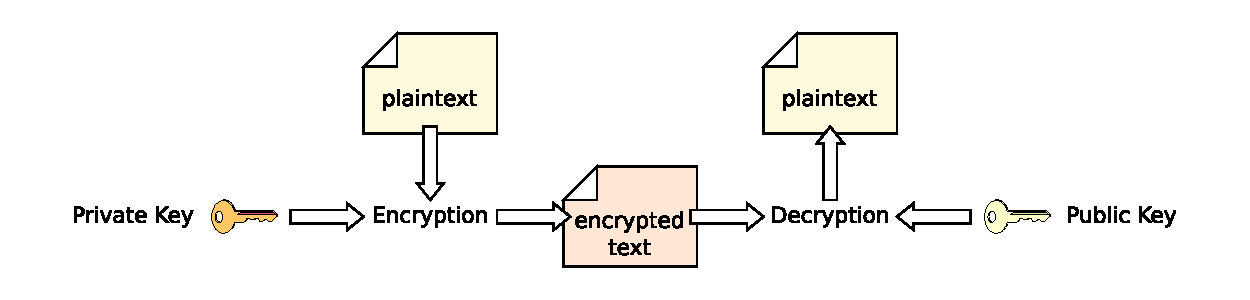
\includegraphics[width=13cm]{tex_tls_echoservice/async.pdf}}\\
	\subfloat[Texttext\label{fig:cgd}]
		{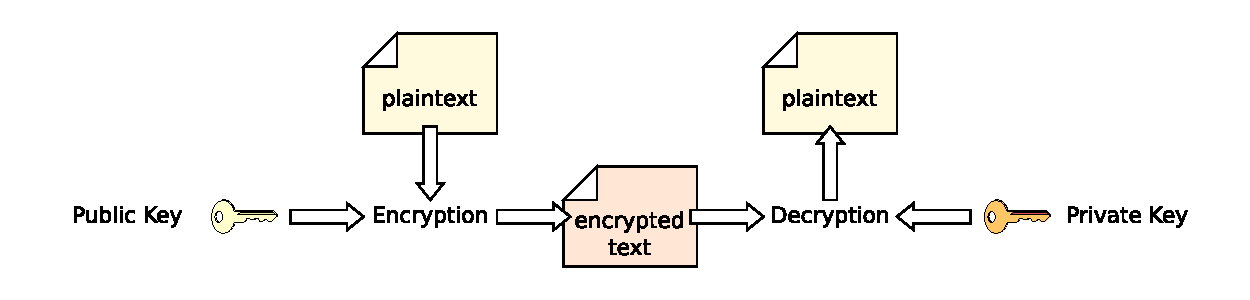
\includegraphics[width=13cm]{tex_tls_echoservice/async2.pdf}}

	\mycaption{specific}{general}
\label{fig:HED_internal0}
\end{figure}


\begin{figure}[htb]
	\centering%epstopdf certificates.eps
 	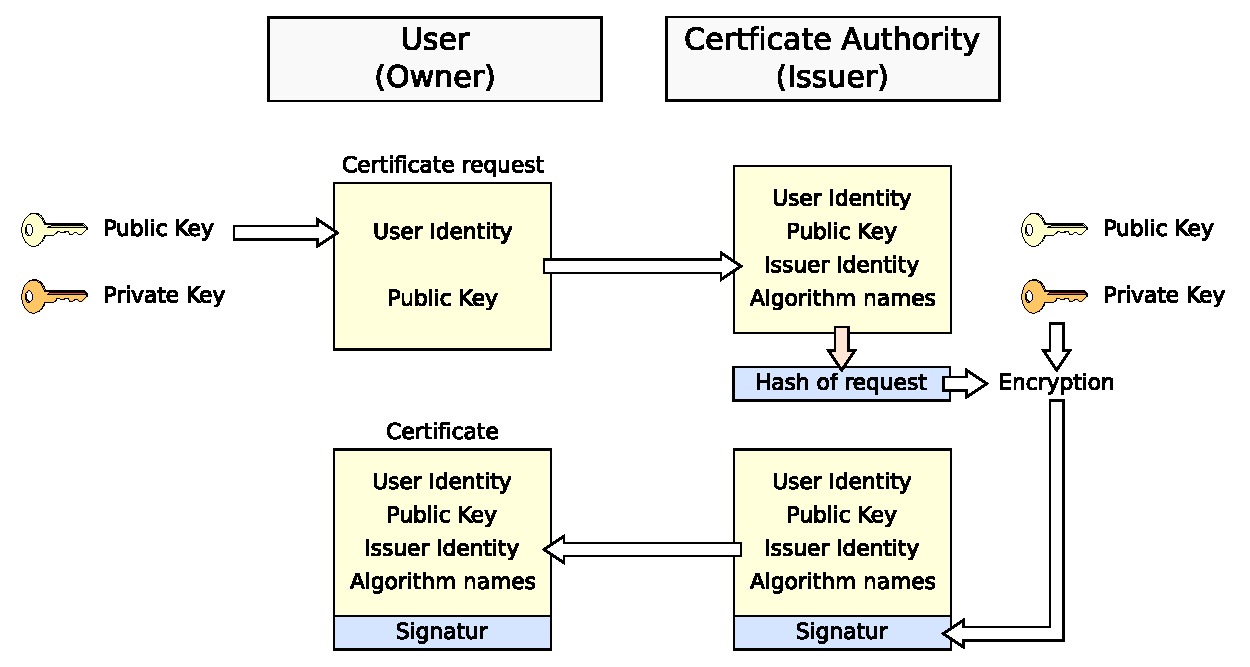
\includegraphics[width=13cm]{tex_tls_echoservice/certificates.pdf}
	\mycaption{specific}{general}
\label{fig:HED_internal2}
\end{figure}

4 types:
                <KeyPath>./clientKey.pem</KeyPath>
                <CertificatePath>./clientCert.pem</CertificatePath>
                <CACertificatePath>./serviceCA.pem</CACertificatePath>


clientCA   - Authority guarantee for identity
clientCERT - Certificate given
clientKEY  - Secret key of the client to read messages, encrypted by the public key in the certificate!

serverCA   - Authority guarantee for cert. CA is known by the server. If not, the encrypted cert can be read be its CA.
serverCERT - Certificate given by the CA. Contains a snippet which can be read by the Public key of the CA.
serverKEY  - Secret key of the client to read messages, encrypted by the public key in the certificate!

\begin{figure}[htb]
	\centering%epstopdf verification.eps 
	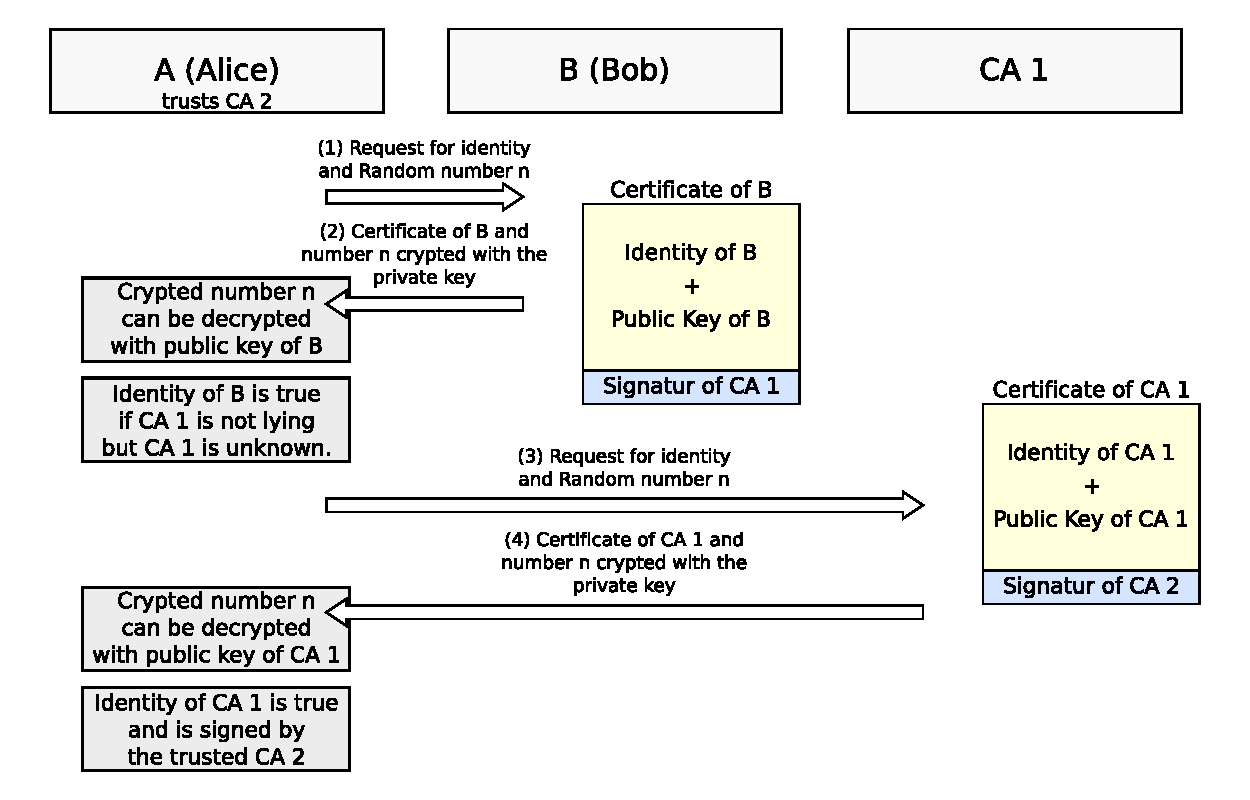
\includegraphics[width=13cm]{tex_tls_echoservice/verification.pdf}
	\mycaption{specific}{general}
\label{fig:HED_internal3}
\end{figure}
Server has got have:
Its  serverCERT serverKEY and some kind of root CA knowing the client
Client has got to have
Its  clientCERT clientKEY and some kind of root CA knowing the server


WARNING: If the programm fails, check if one of your certifacte is expired. If so, create new one using the script files in the directory 'certFactory'

For HED is build up to  % entsrprechend einer Mod Structur
be modular, the security can easily be extend to our given example.
Each Message Chain Component (MCC) or service has a common interface for implementing various pluggable components (plug-ins) called SecHandler. The SecHandler components provide a method for processing messages traveling through Message Chains of the HED. 
Each MCC or Service usually implement two queues of SecHandlers – one for incoming messages and one for outgoing called “incoming” and “outgoing” respectively. All SecHandler components attached to the queue are executed sequentially. 
If any of them fails, message processing fails as well. 
Each SecHandler is configured inside the arched configuration file used for configuring whole chain of MCCs 
Some of the currently implemented SecHandler components make use of pluggable and configurable sub-modules called Policy Decision Point (PDP). PDP can process ARC specific Request and Policy documents which are as well written in XML format~\cite{QIANG_2008}..



\lstsetCPP
\lstinputlisting
	[
	label=lst:arcecho_arched_xml,float,
	caption={[HED configuration file for the Arc intern echo service. Filename: arcecho\_no\_ssl.xml]
	\textbf{HED configuration file for the Arc intern echo service. Filename: arcecho\_no\_ssl.xml\textcolor{white}{hmf}}}
	]
{../src/clients/tlsechoclient/tlsechoclient.cpp}



\lstsetCPP
\lstinputlisting
	[
	label=lst:arcecho_arched_xml,float,
	caption={[HED configuration file for the Arc intern echo service. Filename: arcecho\_no\_ssl.xml]
	\textbf{HED configuration file for the Arc intern echo service. Filename: arcecho\_no\_ssl.xml\textcolor{white}{hmf}}}
	]
{../src/services/tlsechoservice/tlsechoservice.cpp}




\lstsetARCHEDXML
\lstinputlisting
	[
	label=lst:arcecho_arched_xml,float,
	caption={[HED configuration file for the Arc intern echo service. Filename: arcecho\_no\_ssl.xml]
	\textbf{HED configuration file for the Arc intern echo service. Filename: arcecho\_no\_ssl.xml\textcolor{white}{hmf}}}
	]
{../src/services/tlsechoservice/arched_tls_echoservice.xml}



\lstsetKSH
\begin{lstlisting}[
label=lst:invokation_arched_timeservice,float,
caption={[Transformation in eine uniforme konzentrische Verteilung.]
         \textbf{Transformation in eine uniforme konzentrische Verteilung.\textcolor{white}{hmf}}}]
$ rm -f /var/log/arched.log
$ arched -c arched_echoservice.xml  && echo jo ||echo n
$ tail -n100 -f /var/log/arched.log
$ killall arched
\end{lstlisting}



\lstsetKSH
\begin{lstlisting}[
label=lst:invokation_arched_timeservice,float,
caption={[Transformation in eine uniforme konzentrische Verteilung.]
         \textbf{Transformation in eine uniforme konzentrische Verteilung.\textcolor{white}{hmf}}}]
$ ./echoclient
Tue Feb 17 17:04:08 2009
\end{lstlisting}






\lstsetJUSTXML
\begin{lstlisting}[
label=lst:timeservice_cpp_source,float,
caption={[Transformation in eine uniforme konzentrische Verteilung.]
         \textbf{Transformation in eine uniforme konzentrische Verteilung.\textcolor{white}{hmf}}}]
<soap-env:Envelope xmlns:echo="urn:echo" xmlns:soap-enc="http://schemas.xmlsoap.org/soap/encoding/" xmlns:soap-env="http://schemas.xmlsoap.org/soap/envelope/" xmlns:xsd="http://www.w3.org/2001/XMLSchema" xmlns:xsi="http://www.w3.org/2001/XMLSchema-instance">
	<soap-env:Body>
		<echoRequest:echo>
			<echo:say>Der_Berg_ruft</echo:say>
		</echoRequest:echo>
	</soap-env:Body>
</soap-env:Envelope>
\end{lstlisting}



\lstsetJUSTXML
\begin{lstlisting}[
label=lst:timeservice_cpp_source,float,
caption={[Transformation in eine uniforme konzentrische Verteilung.]
         \textbf{Transformation in eine uniforme konzentrische Verteilung.\textcolor{white}{hmf}}}]
<soap-env:Envelope xmlns:echo="urn:echo" xmlns:soap-enc="http://schemas.xmlsoap.org/soap/encoding/" xmlns:soap-env="http://schemas.xmlsoap.org/soap/envelope/" xmlns:xsd="http://www.w3.org/2001/XMLSchema" xmlns:xsi="http://www.w3.org/2001/XMLSchema-instance">
  <soap-env:Body>
    <echo:echoResponse>
      <echo:hear>[ Der_Berg_ruft ]</echo:hear>
    </echo:echoResponse>
  </soap-env:Body>
</soap-env:Envelope>
\end{lstlisting}

